\documentclass[12p,a4paper]{article}
\usepackage[utf8]{inputenc}
\usepackage[T1]{fontenc,url}
\usepackage{multicol}
\usepackage{multirow}
\usepackage{parskip}
\usepackage{lmodern}
\usepackage{microtype}
\usepackage{verbatim}
\usepackage{amsmath, amssymb}
\usepackage{tikz}
\usepackage{physics}
\usepackage{mathtools}
\usepackage{algorithm}
\usepackage{algpseudocode}
\usepackage{listings}
\usepackage{enumerate}
\usepackage{graphicx}
\usepackage{float}
\usepackage{hyperref}
\usepackage{tabularx}
\usepackage{siunitx}
\usepackage{fancyvrb}
\usepackage[makeroom]{cancel}
\usepackage[margin=2cm]{geometry}
\setlength\parindent{0pt}
\renewcommand{\baselinestretch}{1}

\newcommand{\half}{\frac{1}{2}}
\renewcommand{\b}{\boldsymbol}
\newcommand{\h}{\hat}
\newcommand{\m}{\mathbb}
\newcommand{\0}{\ket{0}}
\newcommand{\1}{\ket{1}}
\renewcommand{\exp}{e^}


\begin{document}

\title{FYS3110 -- Home Exam}
\author{
    \begin{tabular}{r l}
        Candidate Number 15229
    \end{tabular}}

\maketitle




\section*{Problem 1}
\subsection*{1.1}
\begin{align*}
    \sigma_x \0 = \begin{pmatrix} 0 & 1 \\ 1 & 0 \end{pmatrix} \begin{pmatrix} 0 \\ 1 \end{pmatrix}
    = \begin{pmatrix} 0 \cdot 0 + 1 \cdot 1 \\ 1 \cdot 0 + 0 \cdot 1 \end{pmatrix}
    = \begin{pmatrix} 1 \\ 0 \end{pmatrix} = \1
\end{align*}

\begin{align*}
    \sigma_x \1 = \begin{pmatrix} 0 & 1 \\ 1 & 0 \end{pmatrix} \begin{pmatrix} 1 \\ 0 \end{pmatrix}
    = \begin{pmatrix} 1 \cdot 0 + 0 \cdot 1 \\ 1 \cdot 1 + 0 \cdot 0 \end{pmatrix}
    = \begin{pmatrix} 0 \\ 1 \end{pmatrix} = \0
\end{align*}
We see that the Pauli x-spin matrix $\sigma_x$ acting on a spin in z-direction, flips the spin to the oposite value.


\subsection*{1.2}
Our requirement that both $\ket{o} = G\ket{i}$ and $\ket{i} = G\ket{o}$ holds, means that
\begin{align*}
    \ket{o} = G\ket{i} = GG\ket{o}
\end{align*}
Since $\ket{o} = GG\ket{o}$, $GG$ must act as the identity operator, giving that G is unitary:
\begin{align*}
    GG = I \quad \rightarrow \quad G = G^{-1}
\end{align*}

If G were a hermitian operator, the following would hold:
\begin{align*}
    \bra{i}G\ket{o} = \bra{o}G\ket{i}
\end{align*}
Inserting for $G\ket{o} = \ket{i}$ and $G\ket{i} = \ket{o}$, we get that
\begin{align*}
    \bra{i}\ket{i} = \bra{o}\ket{o}
\end{align*}
Since $G$ is meant to "preserve normalization", it is natural to asume that $\ket{o}$ and $\ket{i}$ are normalized to 1, and the statement above holds. Since it holds, $G$ must be hermitian.



\subsection*{1.3}
We have defined our qubit basis states to be the z spin-up and spin-down states. We have in exercise 1.1 observed that the Pauli x-spin matrix switches the z-spin basis states. We can therefore represent a NOT gate through a $\sigma_x$ operator.

If $\sigma_x$ is hermitian, it should hold that $\sigma_x^\dag = \sigma_x$. We see that
\begin{align*}
    \sigma_x^\dag = (\sigma_x^T)^* = \begin{pmatrix} 0 & 1 \\ 1 & 0 \end{pmatrix} = \sigma_x
\end{align*}

If $\sigma_x$ is unitary, it should hold that $\sigma_x^2 = I$:
\begin{align*}
    \sigma_x^2 = \begin{pmatrix} 0 & 1 \\ 1 & 0 \end{pmatrix} \begin{pmatrix} 0 & 1 \\ 1 & 0 \end{pmatrix} = \begin{pmatrix} 1 & 0 \\ 0 & 1 \end{pmatrix} = I
\end{align*}

We can see that $\sigma_x$ is both unitary and hermitian.



\subsection*{1.4}
I choose to refer to the gate operator as $H_g$, to reserve $H$ for the hamiltonian operator, for later usage.

If $H_g$ is unitary, it should hold that $H_g^2 = I$:
\begin{align*}
    H_g^2 =
    \frac{1}{\sqrt{2}} \begin{pmatrix} 1 & 1 \\ 1 & -1 \end{pmatrix} \frac{1}{\sqrt{2}} \begin{pmatrix} 1 & 1 \\ 1 & -1 \end{pmatrix}
    = \frac{1}{\sqrt{2}} \begin{pmatrix} 1\cdot 1 + 1\cdot 1 & 1\cdot 1 + 1\cdot(-1) \\ 1\cdot 1 + (-1)\cdot 1 & 1\cdot 1 + (-1)\cdot(-1) \end{pmatrix} = \begin{pmatrix} 1 & 0 \\ 0 & 1 \end{pmatrix} = I
\end{align*}

If $H_g$ is hermitian, it should hold that $H_g^\dag = H_g$:
\begin{align*}
    H_g^\dag = \frac{1}{\sqrt{2}}\qty(\begin{pmatrix} 1 & 1 \\ 1 & -1 \end{pmatrix}^T)^* = \frac{1}{\sqrt{2}}\begin{pmatrix} 1 & 1 \\ 1 & -1 \end{pmatrix}^* = \frac{1}{\sqrt{2}}\begin{pmatrix} 1 & 1 \\ 1 & -1 \end{pmatrix} = H_g
\end{align*}

We see that $H_g$ is both hermitian and unitary.

Applying $H_g$ upon the basis states gets us
\begin{align*}
    H_g\ket{0} = \frac{1}{\sqrt{2}}\begin{pmatrix} 1 & 1 \\ 1 & -1 \end{pmatrix}\begin{pmatrix} 0 \\ 1 \end{pmatrix} = \frac{1}{\sqrt{2}}\begin{pmatrix} 1 \\ -1 \end{pmatrix} = \frac{1}{\sqrt{2}}\qty(\ket{1} - \ket{0})
\end{align*}

\begin{align*}
    H_g\ket{1} = \frac{1}{\sqrt{2}}\begin{pmatrix} 1 & 1 \\ 1 & -1 \end{pmatrix}\begin{pmatrix} 1 \\ 0 \end{pmatrix} = \frac{1}{\sqrt{2}}\begin{pmatrix} 1 \\ 1 \end{pmatrix} = \frac{1}{\sqrt{2}}\qty(\ket{1} + \ket{0})
\end{align*}

We see that applying $H_g$ to the basis states gives us a superposition of the two states. We recongize these superpositions as the up and down spins in the x-direction. The $H_g$ gate turns the z up-spin into an x up-spin, and the z down-spin into an x down-spin.


\subsection*{1.5}
We will implement the H-gate as a magnetic field, $\vec{B}$, turned on for a duration $t_1$. The time-evolution of a 1/2-spin state (here in the spin-z basis) is governed by
\begin{align}\label{eqn:time}
    \chi_z(t) = \alpha\exp{-iE_+t/\hbar}\ket{+} + \beta\exp{-E_-t/\hbar}\ket{-}
\end{align}
Here, $\ket{+}$ and $\ket{-}$ are the eigenstates of the 1/2-spin systems Hamiltonian in the spin-z basis, and $E_+$ and $E_-$ are their respective eigenvalues(the observed energies of the eigenstates).

The Hamiltonian, $H$, of a 1/2-spin particle in a magnetic field $\vec{B}$ is\footnote{I will refer to the Hamiltonian as $H$, and the gate-operator as $H_g$.}
\begin{align*}
    H = -\gamma \vec{B}\cdot \vec{S}
\end{align*}
where $\vec{S} = [S_x, S_y, S_z] = \frac{\hbar}{2}[\sigma_x, \sigma_y, \sigma_z]$, where $\sigma_i$ are the Pauli spin matrices. This gives the Hamiltonian
\begin{align*}
    H = -\gamma \frac{\hbar}{2}\ [B_x \sigma_x,\ B_y \sigma_y,\ B_z \sigma_z]
\end{align*}
If we wish this to be an implementation of the $H_g$-gate, they must share a common set of eigenstates. To achive this, we wish to write $H$ as constant times the $H_g$ operator. Since $\sigma_y$ is the only Pauli spin-matrix containing complex terms, we remove it by setting $B_y = 0$. Further, we see that
\begin{align*}
    H_g = \begin{pmatrix} 1 & 1 \\ 1 & -1 \end{pmatrix} = \frac{1}{\sqrt{2}}(\sigma_x + \sigma_z)
\end{align*}
This means that the magnetic fields in x and z direction must be of equal strength, and we require that
\begin{align*}
    B_z = B_x = B_0
\end{align*}
Since the strength of the magnetic field should equal $h$, we get that
\begin{align*}
    |\vec{B}| = h = \sqrt{B_0^2 + B_0^2} \quad \rightarrow \quad B_0 = \frac{h}{\sqrt{2}}
\end{align*}
We have now chosen a magnetic field in x-z direction, with equal stregth in each of these directions.

By forcing the Hamiltonian to be written in terms of $H_g$, we get
\begin{align*}
    H = -\gamma \frac{\hbar h}{2} H_g
\end{align*}

To solve for time-dependency, we need the Hamiltonians eigenstates and -values. This is left to Wolfram Alpha, and results in the states and energies
\begin{align*}
    \ket{+} &= \begin{pmatrix} 1 - \sqrt{2} \\ 1 \end{pmatrix}\quad\quad E_+ = \gamma\frac{\hbar h}{2} \\
    \ket{-} &= \begin{pmatrix} 1 + \sqrt{2} \\ 1 \end{pmatrix}\quad\quad E_- = -\gamma\frac{\hbar h}{2}
\end{align*}

Inserting this into equation \ref{eqn:time} gives
\begin{align*}
    \chi_z(t) = \alpha \exp{it'}\begin{pmatrix} 1 - \sqrt{2} \\ 1 \end{pmatrix}  + \beta \exp{-it'}\begin{pmatrix} 1 + \sqrt{2} \\ 1 \end{pmatrix}
\end{align*}
where we have introduced $t' = \gamma\frac{h}{2}t$

We will now solve the duration of which the field must be turned on. This is done for both the spin-up and spin-down state, seperately.


\subsubsection*{The up-state}
Knowing that the z-spin is purely upwards at $t=0$ gives us the criteria
\begin{align*}
    \chi_z(0) = \alpha \begin{pmatrix} 1 - \sqrt{2} \\ 1 \end{pmatrix}  + \beta \begin{pmatrix} 1 + \sqrt{2} \\ 1 \end{pmatrix} = \begin{pmatrix} 1 \\ 0 \end{pmatrix}
\end{align*}
This is two equations with two unknowns, and is left to Wolfram Alpha. It requires that
\begin{align*}
    \alpha = -\frac{1}{2\sqrt{2}}\quad\quad \beta = \frac{1}{2\sqrt{2}}
\end{align*}
This gives us the time-expansion
\begin{align*}
    \chi_z(t) = -\frac{1}{2\sqrt{2}} \exp{it'}\begin{pmatrix} 1 - \sqrt{2} \\ 1 \end{pmatrix}  + \frac{1}{2\sqrt{2}} \exp{-it'}\begin{pmatrix} 1 + \sqrt{2} \\ 1 \end{pmatrix}
\end{align*}

We require that this, at some point $t'=t_1'$, becomes the x-spin-up state, represented as $\frac{1}{\sqrt{2}}\begin{pmatrix} 1 \\ 1 \end{pmatrix}$ in the spin-z basis. This results in two equation, and we pick out the "second" one (second components in the vector equation). The equations also carry a global phase-factor, which we will just add at the end, when we need it.
\begin{align*}
    -\frac{1}{2\sqrt{2}}\exp{it_1'} + \frac{1}{2\sqrt{2}}\exp{-it_1'} = \frac{1}{\sqrt{2}}
\end{align*}
Using Eulers formula and multiplying with $2\sqrt{2}$ gives
\begin{align*}
    -\cos(t_1') -i\sin(t_1') = \cos(-t_1') + i\sin(-t_1') = 2
\end{align*}
Since we know that $\cos(-x) = \cos(x)$ and $\sin(-x) = -\sin(x)$, we get
\begin{align*}
    -i\sin(t_1') = 1
\end{align*}
Since we would very much like to have a non-complex time, we require that our global phase factor $\exp{i\theta} = \pm i$, as any other choice would introduce a complex component. Since we would also like our time to be positive, we pick the sign on the phase factor such that
\begin{align*}
    -i\sin(t_1') = 1\cdot \exp{i\theta} = -i \\
    \sin(t_1') = 1 \\
    t_1' = 2\pi n + \frac{\pi}{2}
\end{align*}
for $n\in {0,1,2,3...}$.\\
Inserting for $t_1'$ and considering that we would probably like the the duration of the magnetic field to be as short as possible (i.e. $n = 0$), and Inserting for $\gamma = g\frac{\mu_B}{\hbar} = \frac{ge}{2m}$, we get the duration
\begin{align*}
    t_1 = \frac{2t_1'}{h\gamma} = \frac{\pi}{h\gamma} = \frac{2\pi m}{h g e}
\end{align*}


\subsubsection*{The spin-down state}
We will now, hopefully, solve for the same time in the spin-down state.

Knowing that the z-spin is purely downwards at $t=0$ gives us the criteria
\begin{align*}
    \chi_z(0) = \alpha \begin{pmatrix} 1 - \sqrt{2} \\ 1 \end{pmatrix}  + \beta \begin{pmatrix} 1 + \sqrt{2} \\ 1 \end{pmatrix} = \begin{pmatrix} 0 \\ 1 \end{pmatrix}
\end{align*}
This is, again, left to Wolfram Alpha, giving the coefficients
\begin{align*}
    \alpha = \frac{\sqrt{2}+1}{2\sqrt{2}}\quad\quad \beta = \frac{\sqrt{2}-1}{2\sqrt{2}}
\end{align*}
This gives us the time-expansion
\begin{align*}
    \chi_z(t) = \frac{\sqrt{2}+1}{2\sqrt{2}} \exp{it'}\begin{pmatrix} 1 - \sqrt{2} \\ 1 \end{pmatrix}  + \frac{\sqrt{2}-1}{2\sqrt{2}} \exp{-it'}\begin{pmatrix} 1 + \sqrt{2} \\ 1 \end{pmatrix}
\end{align*}

We require that this, at some point $t'=t_1'$, becomes the x-spin-down state, represented as $\frac{1}{\sqrt{2}}\begin{pmatrix} 1 \\ -1 \end{pmatrix}$ in the spin-z basis. This results in two equation, and we pick out with the "first" one. The phase factor will again be considered at the end.
\begin{align*}
    \frac{\sqrt{2}+1}{2\sqrt{2}} \exp{it_1'}(1 - \sqrt{2})  + \frac{\sqrt{2}-1}{2\sqrt{2}} \exp{-it_1'}(1 + \sqrt{2}) = \frac{1}{\sqrt{2}}\begin{pmatrix} 1 \\ -1 \end{pmatrix}
\end{align*}
Multiplying by $2\sqrt{2}$, writing out all the terms, and using Eulers formula, gives
\begin{align*}
    -\cos(t_1') -i\sin(t_1') = \cos(-t_1') + i\sin(-t_1') = 2
\end{align*}

We see that this is exactly the same we got in the spin-up state. Using the same approach, we will obviously arrive at the same time for the spin-down as we did for the spin-up. This is a great sign that our solution is probably correct. It's also rather convenient to have the $\vec{B}$-field on for the same duration, regardless of wether we wish to flip a spin-up or spin-down particle. Anything else would be somewhat impractical to implement.

To sum up, our implementation of the $H_g$-gate is a $\vec{B} = \frac{h}{\sqrt{2}}\vec{i_x} + \frac{h}{\sqrt{2}}\vec{i_z}$ field, turned on for a duration $ t_1 = \frac{2\pi m}{h g e}$.

\section*{Problem 2}
\subsection*{2.1}
We have a set of $N$ integers, and apply an operator $f$, which will return True at a specific integer $i^*$. We will call $n$ the number of times we had to apply $f$ in order to figure out $i^*$, and it ranges anywhere between $1$ and $N$.\footnote{Technically, when we have applied $f$ $N-1$ times, we know that $i^*$ must be the last integer, and do not need to apply $f$ one last time. However, if we consider cases of large $N$s, this case is negligible. We could also say that we \textit{must} apply $f$ also the $N$'th time, 'just to be sure' that the last value is actually $i^*$.} The probability that we will find $i^*$ after $n$ applications of $f$, is uniformly equal to $1/N$:\footnote{We are considering the probability of needing exactly $n$ applications of $f$ from the start of. If we have already made $n-1$ applications of $f$, the probability of finding $i^*$ at the $n$'th applications would be different, but this is not the probability we are looking for. Looking at the system from before any applications, each 'guess' is equally probable of giving us $i^*$.}
\begin{align*}
    P(n) = \frac{1}{N}
\end{align*}
The expectation value of the number of guesses needed to find $i^*$ is then given as
\begin{align*}
    \langle n \rangle = \sum\limits_{n=1}^N n\ P(n) = \frac{1}{N}\sum\limits_{n=1}^N n = \frac{1}{N}\qty(\frac{N(N+1)}{2}) = \frac{N+1}{2}
\end{align*}



\subsection*{2.2}
Applying the operator $F = I - 2 \ket{i^*}\bra{i^*}$ onto a state $\ket{i}$ gives.
\begin{align*}
    F\ket{i} = I\ket{i} - 2 \ket{i^*}\bra{i^*}\ket{i}
\end{align*}

For cases $\ket{i} \neq \ket{i^*}$, the orthogonality of the states $\ket{i}$ gives $\bra{i^*}\ket{i} = 0$, which means that we get the expected behavior from $F$:
\begin{align*}
    F\ket{i} = I\ket{i} - 0 = \ket{i}
\end{align*}

For cases $\ket{i} = \ket{i^*}$, the normality of the states $\ket{i}$ means that $\bra{i^*}\ket{i^*} = 1$, which again gives us the expected behavior from $F$:
\begin{align*}
    F\ket{i^*} = I\ket{i^*} - 2\ket{i^*}\cdot 1 = -\ket{i^*}
\end{align*}
We see that the chosen representation of the operator $F$ behaves as expected.

If $F$ is an unitary operator, the must hold that $F^2 = I$:
\begin{align*}
    F^2 = (I - 2\ket{i^*}\bra{i^*})^2 = I - 4\ket{i^*}\bra{i^*} + 4\ket{i^*}\bra{i^*}\ket{i^*}\bra{i^*} = I - 4\ket{i^*}\bra{i^*} + 4\ket{i^*}\bra{i^*} = I
\end{align*}
due to the normalization of $i^*$, giving $\bra{i^*}\ket{i^*} = 1$.

For $F$ to be hermitian, we require that $F^\dag = F$
\begin{align*}
    F^\dag = (I - 2\ket{i^*}\bra{i^*})^\dag = I^\dag - 2(\ket{i^*}\bra{i^*})^\dag = I - 2\ket{i^*}\bra{i^*} = I
\end{align*}

We see that $F$ is both unitary and hermitian.

\subsection*{2.3}
For $\bra{i^*}\ket{s}$, we get that
\begin{align*}
    \bra{i^*}\ket{s} = \bra{i^*}\frac{1}{\sqrt{N}}\sum\limits_{i=1}^N \ket{i} = \frac{1}{\sqrt{N}}\sum\limits_{i=1}^N \bra{i^*}\ket{i}
\end{align*}
The inner product $\bra{i^*}\ket{i}$ will, due to the orthonormality of the $\ket{i}$s, be 0 for all cases but $\bra{i^*}\ket{i^*}$, where it will be 1. The sum simply evaluates to 1, giving
\begin{align}\label{eqn:i*s}
    \bra{i^*}\ket{s} = \frac{1}{\sqrt{N}}
\end{align}

For $F\ket{s}$, we get that
\begin{align*}
    F\ket{s} = (I - 2\ket{i^*}\bra{i^*})\ket{s} = I\ket{s} - 2 \ket{i^*}\bra{i^*}\ket{s}
\end{align*}
Using \ref{eqn:i*s}, this becomes
\begin{align*}
    F\ket{s} = \ket{s} - \frac{2}{\sqrt{N}}\ket{i^*}
\end{align*}



\subsection*{2.4}
We demand that $\ket{g}$ is normalized, meaning that
\begin{align*}
    \bra{g}\ket{g} = 1 = \big[\bra{s}\alpha^* + \bra{i^*}\beta^*] \cdot \big[\alpha\ket{s} + \beta\ket{i^*}] \\
    = \alpha^2 \bra{s}\ket{s} + 2\alpha\beta\bra{i^*}\ket{s} + \beta^2\bra{i^*}\ket{i^*}
\end{align*}
Using that $\ket{i^*}$ and $\ket{s}$ are normalized, and applying the inner product from last exercise, we get that
\begin{align*}
    \alpha^2 + \beta^2 + \frac{2}{\sqrt{N}}\alpha\beta = 1
\end{align*}
which is our normalization condition.



\subsection*{2.5}
The operator $X$ represents a spectral representation of the eigenvalues of $\ket{i}$.

Applying the given $X$ operator onto a state $\ket{i}$ gives us
\begin{align*}
    X\ket{i} = \sum\limits_{j=1}^N j\ket{j}\bra{j}\ket{i}
\end{align*}
Due to the orthogonality of the states, only the $j=i$ term of the sum is non-zero, and we get
\begin{align*}
    X\ket{i} = i\ket{i}
\end{align*}
We see that any state $\ket{i}$ is an eigenstate of $X$, and gives us an eigenvalue, representing an observation of the state. Since the operator retrives the observable quantity of $\ket{i}$, we can accurately consider it an observation of $i$.



\subsection*{2.6}
Since the states are non-degenerate, we can simply multiply $\bra{i^*}$ from the right and square to get the probability of measuring $i$.
\begin{align*}
    P(i^*) = \qty(\bra{i^*}\ket{g})^2 = \qty(\alpha\bra{i^*}\ket{s} +\beta\bra{i^*}\ket{i^*})^2 = \qty(\frac{\alpha}{\sqrt{N}} + \beta)^2 = \frac{\alpha^2}{N} + 2\frac{\alpha\beta}{\sqrt{N}} + \beta^2
\end{align*}
We recognize the last two terms from exercise 2.4, where we can rewrite the normalization condition as $2\frac{\alpha\beta}{\sqrt{N}} + \beta^2 = \alpha^2 - 1$, which gives
\begin{align*}
    P(i^*) = \frac{\alpha^2}{N} + 1 - \alpha^2 = \alpha^2\qty(\frac{1}{N} - 1) + 1
\end{align*}



\subsection*{2.7}
\begin{align*}
    UF\ket{s} &= U\qty(\ket{s} - \frac{2}{\sqrt{N}}\ket{i^*}) = U\ket{s} - \frac{2}{\sqrt{N}}U\ket{i^*}\\
    &= 2\ket{s}\bra{s}\ket{s} - I\ket{s} - \frac{2}{\sqrt{N}}(2\ket{s}\bra{s}\ket{i^*} - I\ket{i^*}) \\
    &= \ket{s} - \frac{4}{N}\ket{s} + \ket{i^*} = \qty(1 - \frac{4}{N})\ket{s} + \frac{2}{\sqrt{N}}\ket{i^*}
\end{align*}

The norm of $UF\ket{s}$ becomes
\begin{align*}
    |UF\ket{s}|^2 = \bra{s}F^\dag U^\dag U F\ket{s} = \bra{s}F U U F\ket{s}
\end{align*}
We can see that $U$ is also unitary
\begin{align*}
    U^2 = (2\ket{s}\bra{s} - I)^2 = 4\ket{s}\bra{s}\ket{s}\bra{s} - 4\ket{s}\bra{s} + I = 4\ket{s}\bra{s} - 4\ket{s}\bra{s} + I = I
\end{align*}
Iserting both $UU = I$ and $FF = I$, we get that
\begin{align*}
    |UF\ket{s}|^2 = \bra{s}F U U F\ket{s} = \bra{s}FF\ket{s} = \bra{s}\ket{s} = 1
\end{align*}
giving that $UF\ket{s}$ is normalized.



\subsection*{2.8}Writing out $UF$ becomes
\begin{align*}
    UF = (2\ket{s}\bra{s} - I)(I - 2\ket{i^*}\bra{i^*}) = 2\ket{s}\bra{s} + 2\ket{i^*}\bra{i^*} - \frac{4}{\sqrt{N}}\ket{s}\bra{i^*} - I
\end{align*}

We already know that $UF\ket{s} = \qty(1 - \frac{4}{N})\ket{s} + \ket{i^*}$. Applying this, we get that
\begin{gather*}
    UF(\alpha\ket{s} + \beta\ket{i^*}) = \alpha UF\ket{s} + \beta UF\ket{i^*}\\
    = \alpha\qty(1 - \frac{4}{N})\ket{s} + \alpha\ket{i^*} + \beta\qty[2\ket{s}\bra{s}\ket{i^*} + 2\ket{i^*}\bra{i^*}\ket{i^*} - \frac{4}{\sqrt{N}}\ket{s}\bra{i^*}\ket{i^*} - I\ket{i^*}]\\
    = \alpha\qty(1 - \frac{4}{N})\ket{s} + \alpha\ket{i^*} + \frac{2}{\sqrt{N}}\beta\ket{s} + 2\beta\ket{i^*} - \beta\frac{4}{\sqrt{N}}\ket{s} - \beta\ket{i^*}]\\
    = \qty[\alpha\qty(1-\frac{4}{N}) - \frac{2}{\sqrt{N}}\beta]\ket{s} + \qty[\alpha\frac{2}{\sqrt{N}} + \beta]\ket{i^*}
\end{gather*}



\subsection*{2.9}
Applying $UF$ onto $\ket{s}$ in 2.7, we saw that the result is some linear combination of $\ket{s}$ and $\ket{i^*}$. From 2.8 we know that $UF$ applied onto such a linear combination itself is a linear combination. If we also treat the first product, $UF\ket{s}$ as a special case of $UF\ket{g}$ with $\alpha = 1$ and $beta=0$, this will make for a great for-loop in our program. We simply repeatidly apply $UF$ onto the result, $n$ times, using the formula in 2.8.

Below we see a figure showing the probability of measuring a certain state $\ket{i^*}$ after $n$ applications of $UF$. As we can see, the probability oscilates between 0 and 1, with decreasing frequency as the size of the system increases.
\begin{figure}[H]
    \centering
    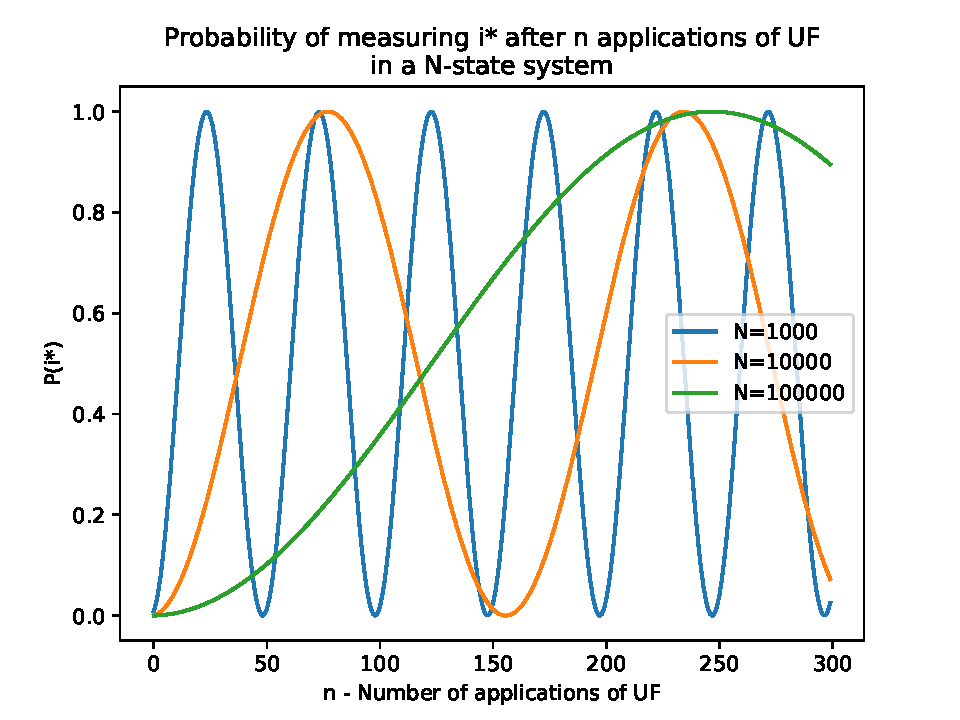
\includegraphics[width=0.8\textwidth]{three_Ns.pdf}
\end{figure}

We introduce $n^*$ as the minumum number of $n$ required to reach $P(i^*) \geq 0.99$ for a specific $N$-system. This value is shown for a set of different $N$'s below.

\begin{tabular}{|c|c|}
    \hline
    $N$	& $n^*$\\
    \hline
    1e2 & 7 \\
	1e3 & 23 \\
	1e4 & 74 \\
	1e5 & 233 \\
	1e6 & 735 \\
	1e7 & 2325 \\
    1e8 & 7353 \\
    \hline
\end{tabular}
\\

Plotting the $n^*$ for a large set of $N$'s, we see a very clear pattern. $n^*$ appears to increase linearly on a logaritmic plot, meaning that it is some exponential function of $N$. The inclination appears to be somewhere around 0.5, meaning $n^* \sim N^{0.5} = \sqrt{N}$.

\begin{figure}[H]
    \centering
    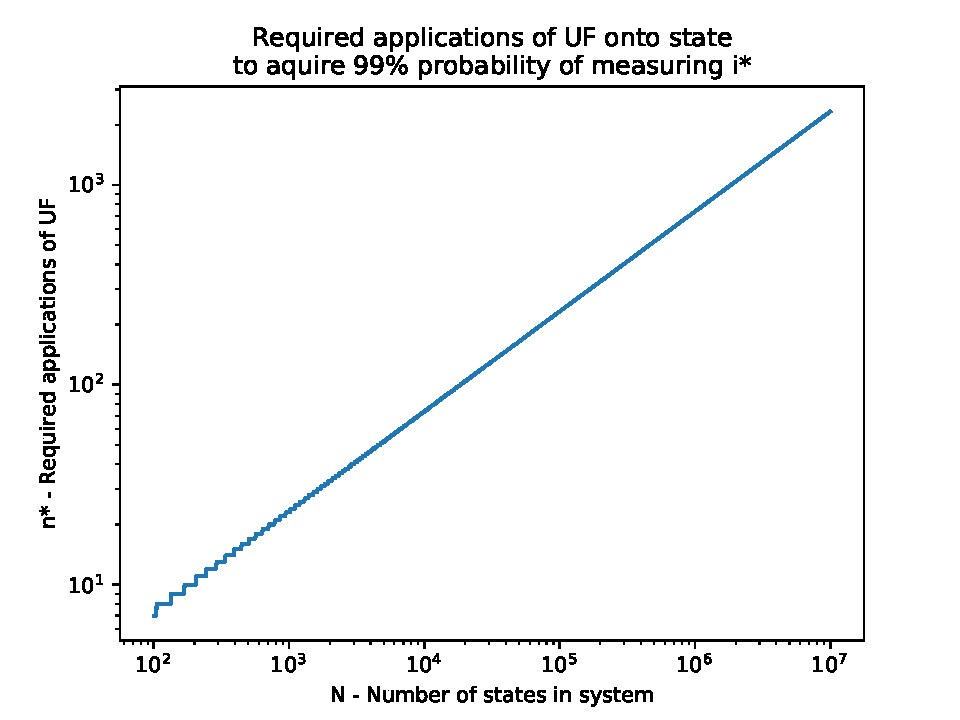
\includegraphics[width=0.8\textwidth]{n_star.pdf}
\end{figure}



\subsection*{2.10}
In the last exercise, I made the guess that $n^*$ is proportional to some exponent of $N$, around 0.5. Going back into our program from 2.9 and doing some linear regression of $\log(n^*)$ against $\log(N)$, we get that the slope of this linear regression is $0.500146429312$. This points heavily towards the assumption that $n^* \sim \sqrt{N}$, with some small margin of error.

So what does this mean? Well, $n^*$ is the \textit{minimum}\footnote{In our calculations of $n^*$, we have chosen our $i^*$ to be the least likely observed state at the begining, and thus the slowest state to observe. We therefore know that no chosen $i^*$ would be slower to observe than $n^*$.} $n$ required for the probability of measuring a specific  $\ket{i^*}$ from a set of $N$ $\ket{i}$s becoming larger than 99\%. Most systems reached far further than this (i.e. 99.99\%) only a few steps after $n^*$. It's therefore not unreasonable to simply consider $n^*$ the number $n$ required for actually observing our chosen state $\ket{i^*}$.

$n$ does itself represent the number of repeated applications of the $UF$ operator onto the system. Since this operator is both hermitian and preserves normalization, it should be perfectly representable as a physical gate in a quantum computer. We also know from 2.1 that we will be capable of differentiating the $\ket{i^*}$ case from the rest of the states through the $F$ operator.

This means that for a set of $N$ $\ket{i}$s (which can represent a database of some values), we can find \textit{any} specific state $\ket{i^*}$ by passing our system through some gate a number of times that scales with $\sqrt{N}$. It's natural to assume that "passing our system through the gate" takes some constant amount of time. We then have a computer which can look for a value $i^*$ in a database of size $N$ in a time that scales with $\sqrt{N}$.



\subsection*{Appendix - 2.9 Code}
\verbatiminput{task2_9.py}


\end{document}
